\PassOptionsToPackage{unicode=true}{hyperref} % options for packages loaded elsewhere
\PassOptionsToPackage{hyphens}{url}
%
\documentclass[]{article}
\usepackage{lmodern}
\usepackage{amssymb,amsmath}
\usepackage{ifxetex,ifluatex}
\usepackage{fixltx2e} % provides \textsubscript
\ifnum 0\ifxetex 1\fi\ifluatex 1\fi=0 % if pdftex
  \usepackage[T1]{fontenc}
  \usepackage[utf8]{inputenc}
  \usepackage{textcomp} % provides euro and other symbols
\else % if luatex or xelatex
  \usepackage{unicode-math}
  \defaultfontfeatures{Ligatures=TeX,Scale=MatchLowercase}
\fi
% use upquote if available, for straight quotes in verbatim environments
\IfFileExists{upquote.sty}{\usepackage{upquote}}{}
% use microtype if available
\IfFileExists{microtype.sty}{%
\usepackage[]{microtype}
\UseMicrotypeSet[protrusion]{basicmath} % disable protrusion for tt fonts
}{}
\IfFileExists{parskip.sty}{%
\usepackage{parskip}
}{% else
\setlength{\parindent}{0pt}
\setlength{\parskip}{6pt plus 2pt minus 1pt}
}
\usepackage{hyperref}
\hypersetup{
            pdftitle={Sesión de Laboratorio: Modelos SARIMA.},
            pdfauthor={Marcelo Molinatti},
            pdfborder={0 0 0},
            breaklinks=true}
\urlstyle{same}  % don't use monospace font for urls
\usepackage[margin=1in]{geometry}
\usepackage{color}
\usepackage{fancyvrb}
\newcommand{\VerbBar}{|}
\newcommand{\VERB}{\Verb[commandchars=\\\{\}]}
\DefineVerbatimEnvironment{Highlighting}{Verbatim}{commandchars=\\\{\}}
% Add ',fontsize=\small' for more characters per line
\usepackage{framed}
\definecolor{shadecolor}{RGB}{248,248,248}
\newenvironment{Shaded}{\begin{snugshade}}{\end{snugshade}}
\newcommand{\AlertTok}[1]{\textcolor[rgb]{0.94,0.16,0.16}{#1}}
\newcommand{\AnnotationTok}[1]{\textcolor[rgb]{0.56,0.35,0.01}{\textbf{\textit{#1}}}}
\newcommand{\AttributeTok}[1]{\textcolor[rgb]{0.77,0.63,0.00}{#1}}
\newcommand{\BaseNTok}[1]{\textcolor[rgb]{0.00,0.00,0.81}{#1}}
\newcommand{\BuiltInTok}[1]{#1}
\newcommand{\CharTok}[1]{\textcolor[rgb]{0.31,0.60,0.02}{#1}}
\newcommand{\CommentTok}[1]{\textcolor[rgb]{0.56,0.35,0.01}{\textit{#1}}}
\newcommand{\CommentVarTok}[1]{\textcolor[rgb]{0.56,0.35,0.01}{\textbf{\textit{#1}}}}
\newcommand{\ConstantTok}[1]{\textcolor[rgb]{0.00,0.00,0.00}{#1}}
\newcommand{\ControlFlowTok}[1]{\textcolor[rgb]{0.13,0.29,0.53}{\textbf{#1}}}
\newcommand{\DataTypeTok}[1]{\textcolor[rgb]{0.13,0.29,0.53}{#1}}
\newcommand{\DecValTok}[1]{\textcolor[rgb]{0.00,0.00,0.81}{#1}}
\newcommand{\DocumentationTok}[1]{\textcolor[rgb]{0.56,0.35,0.01}{\textbf{\textit{#1}}}}
\newcommand{\ErrorTok}[1]{\textcolor[rgb]{0.64,0.00,0.00}{\textbf{#1}}}
\newcommand{\ExtensionTok}[1]{#1}
\newcommand{\FloatTok}[1]{\textcolor[rgb]{0.00,0.00,0.81}{#1}}
\newcommand{\FunctionTok}[1]{\textcolor[rgb]{0.00,0.00,0.00}{#1}}
\newcommand{\ImportTok}[1]{#1}
\newcommand{\InformationTok}[1]{\textcolor[rgb]{0.56,0.35,0.01}{\textbf{\textit{#1}}}}
\newcommand{\KeywordTok}[1]{\textcolor[rgb]{0.13,0.29,0.53}{\textbf{#1}}}
\newcommand{\NormalTok}[1]{#1}
\newcommand{\OperatorTok}[1]{\textcolor[rgb]{0.81,0.36,0.00}{\textbf{#1}}}
\newcommand{\OtherTok}[1]{\textcolor[rgb]{0.56,0.35,0.01}{#1}}
\newcommand{\PreprocessorTok}[1]{\textcolor[rgb]{0.56,0.35,0.01}{\textit{#1}}}
\newcommand{\RegionMarkerTok}[1]{#1}
\newcommand{\SpecialCharTok}[1]{\textcolor[rgb]{0.00,0.00,0.00}{#1}}
\newcommand{\SpecialStringTok}[1]{\textcolor[rgb]{0.31,0.60,0.02}{#1}}
\newcommand{\StringTok}[1]{\textcolor[rgb]{0.31,0.60,0.02}{#1}}
\newcommand{\VariableTok}[1]{\textcolor[rgb]{0.00,0.00,0.00}{#1}}
\newcommand{\VerbatimStringTok}[1]{\textcolor[rgb]{0.31,0.60,0.02}{#1}}
\newcommand{\WarningTok}[1]{\textcolor[rgb]{0.56,0.35,0.01}{\textbf{\textit{#1}}}}
\usepackage{longtable,booktabs}
% Fix footnotes in tables (requires footnote package)
\IfFileExists{footnote.sty}{\usepackage{footnote}\makesavenoteenv{longtable}}{}
\usepackage{graphicx,grffile}
\makeatletter
\def\maxwidth{\ifdim\Gin@nat@width>\linewidth\linewidth\else\Gin@nat@width\fi}
\def\maxheight{\ifdim\Gin@nat@height>\textheight\textheight\else\Gin@nat@height\fi}
\makeatother
% Scale images if necessary, so that they will not overflow the page
% margins by default, and it is still possible to overwrite the defaults
% using explicit options in \includegraphics[width, height, ...]{}
\setkeys{Gin}{width=\maxwidth,height=\maxheight,keepaspectratio}
\setlength{\emergencystretch}{3em}  % prevent overfull lines
\providecommand{\tightlist}{%
  \setlength{\itemsep}{0pt}\setlength{\parskip}{0pt}}
\setcounter{secnumdepth}{5}
% Redefines (sub)paragraphs to behave more like sections
\ifx\paragraph\undefined\else
\let\oldparagraph\paragraph
\renewcommand{\paragraph}[1]{\oldparagraph{#1}\mbox{}}
\fi
\ifx\subparagraph\undefined\else
\let\oldsubparagraph\subparagraph
\renewcommand{\subparagraph}[1]{\oldsubparagraph{#1}\mbox{}}
\fi

% set default figure placement to htbp
\makeatletter
\def\fps@figure{htbp}
\makeatother

\usepackage{amsmath}

\title{Sesión de Laboratorio: Modelos SARIMA.}
\author{Marcelo Molinatti}
\date{2023-03-25}

\begin{document}
\maketitle

{
\setcounter{tocdepth}{2}
\tableofcontents
}
\hypertarget{sesiuxf3n-de-laboratorio-modelos-sarima.}{%
\section{Sesión de Laboratorio: Modelos SARIMA.}\label{sesiuxf3n-de-laboratorio-modelos-sarima.}}

\emph{Marcelo J Molinatti S}

Elija una de las siguientes series temporales estacionales: \texttt{condmilk}, \texttt{hsales}, \texttt{usolec}

\begin{itemize}
\tightlist
\item
  ✅ ¿Es necesario transformar los datos? Si es así, encuentre un transformación adecuado.
\item
  ✅ ¿Son estacionarios los datos? Si no, encuentre una diferenciación apropiada que produce datos estacionarios.
\item
  ✅ Identifique un par de modelos ARIMA que podrían ser útiles en describir la serie de tiempo. ¿Cuál de sus modelos es el mejor de acuerdo con sus valores \(AIC\)?
\item
  ✅ Estime los parámetros de su mejor modelo y haga un diagnóstico de los residuos. ¿Los residuos se parecen al ruido blanco? Si no es así, intente encontrar otro modelo ARIMA que le quede mejor.
\item
  ✅ Pronostique los próximos 24 meses de datos usando su modelo preferido.
\item
  ✅ Compare los pronósticos obtenidos, usando \texttt{ets()}.
\end{itemize}

\hypertarget{descripciuxf3n-de-la-serie.}{%
\subsection{Descripción de la serie.}\label{descripciuxf3n-de-la-serie.}}

\begin{Shaded}
\begin{Highlighting}[]
\CommentTok{# Sourcing R code}
\KeywordTok{source}\NormalTok{(}\StringTok{"../R/Lab-Session-8-FPP.R"}\NormalTok{)}
\end{Highlighting}
\end{Shaded}

Los datos seleccionados corresponden a una serie temporal de Inventarios de Manufactura de leche condensada evaporada y endulzada, recolectados mensualmente desde 1971 a 1980, como se muestra en el gráfico de la figura \ref{fig:tseriesplot}.

\begin{Shaded}
\begin{Highlighting}[]
\CommentTok{# Grafico de la serie temporal}
\KeywordTok{autoplot}\NormalTok{(condmilk, }\DataTypeTok{colour=}\StringTok{"dodgerblue3"}\NormalTok{) }\OperatorTok{+}
\StringTok{  }\KeywordTok{geom_point}\NormalTok{(}\KeywordTok{aes}\NormalTok{(}\DataTypeTok{y=}\NormalTok{value), }\DataTypeTok{colour=}\StringTok{"dodgerblue3"}\NormalTok{) }\OperatorTok{+}\StringTok{ }
\StringTok{  }\KeywordTok{theme_light}\NormalTok{() }\OperatorTok{+}\StringTok{ }
\StringTok{  }\KeywordTok{geom_line}\NormalTok{(}
    \KeywordTok{aes}\NormalTok{(}\DataTypeTok{y=}\KeywordTok{ksmooth}\NormalTok{(}\KeywordTok{time}\NormalTok{(condmilk }\OperatorTok\StringTok{ }\KeywordTok{as.ts}\NormalTok{()), condmilk }\OperatorTok\StringTok{ }\KeywordTok{as.ts}\NormalTok{(), }\StringTok{"normal"}\NormalTok{, }\DataTypeTok{bandwidth=}\NormalTok{.}\DecValTok{5}\NormalTok{)}\OperatorTok{$}\NormalTok{y), }
    \DataTypeTok{colour=}\StringTok{"200"}\NormalTok{, }\DataTypeTok{lwd=}\DecValTok{1}\NormalTok{) }\OperatorTok{+}
\StringTok{  }\KeywordTok{geom_smooth}\NormalTok{(}\KeywordTok{aes}\NormalTok{(}\DataTypeTok{y=}\NormalTok{value), }\DataTypeTok{method=}\NormalTok{loess, }\DataTypeTok{se=}\OtherTok{FALSE}\NormalTok{, }\DataTypeTok{color=}\StringTok{"200"}\NormalTok{, }\DataTypeTok{linetype=}\DecValTok{2}\NormalTok{) }\OperatorTok{+}
\StringTok{  }\KeywordTok{xlab}\NormalTok{(}\StringTok{'Tiempo'}\NormalTok{) }\OperatorTok{+}\StringTok{ }\KeywordTok{ylab}\NormalTok{(}\StringTok{'Numero de Unidades'}\NormalTok{)}
\end{Highlighting}
\end{Shaded}

\begin{center}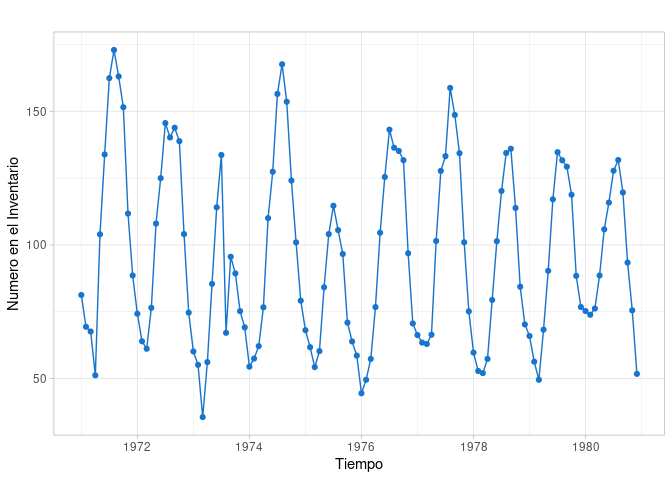
\includegraphics{/home/marcelo/MEGAsync/Msc-Math-Applied/Series Temporales/output/Lab-Session-8-FPP_files/figure-latex/tseries-plot-1} \end{center}

En el gráfico se observa claramente dos componentes estacionales: uno anual obvio, que fluctúa ligeramente, observándose una disrrupción a mediados de 1973 que rompe de alguna manera el patrón unimodal de los picos anuales; y también parece haber un componente trimestral de repeticiones de picos y valles importantes, cuya amplitud disminuye con el tiempo, indicando un amortiguamiento de las variaciones o fluctuaciones importantes en la serie.

Se resaltan en el componente trimestral:
\emph{i)} picos de mayor magnitud cada tres años, a mediados de los años 1971, 1974 y 1977, mostrando un cambio periódico en la amplitud de los ciclos (aunque no se observa pico a mediados de 1980);
\emph{ii)} valles profundos cada 3 años, en los años 1973, 1976 y 1979, con una ligera fluctuación mensual, en donde el número de unidades cae por debajo de las 50 unidades y cuya amplitud, al igual que la de los picos, se va amortiguando cada vez que aparece.

También se observa una pequeña tendencia decreciente durante la primera parte de la serie, que es muy perceptible debido al comportamiento anormal durante el año 1973; pero que desaparece durante la segunda parte de la serie.

\hypertarget{transformaciuxf3n-de-la-serie.}{%
\subsection{Transformación de la serie.}\label{transformaciuxf3n-de-la-serie.}}

Dada la descripción anterior, se decide optar por transformar los datos usando una función logarítmica, con la finalidad de hacer mas obvias las desviaciones importantes que aparecen en la serie; y en lugar de modelar la serie original transformada, se modela la serie que resulta de la diferencia de valores adyacentes (elimina el componente con tendencia en la primer tercio de la serie original):

\[log(x_t) - log(x_{t-1}) = log(\frac{x_t}{x_{t-1}}) = log(1 + r_t)\]

donde \(r_t\) es el incremento o decremento proporcional de la unidad en el año \(t\) con respecto al valor en el año anterior, \(t-1\). Dado que la magnitud de \(r_t\) es pequeña, se puede aproximar \(log(1 + r_t) \approx r_t\). La serie \(r_t\) se muestra en la figura \ref{fig:transform}.

\begin{Shaded}
\begin{Highlighting}[]
\KeywordTok{autoplot}\NormalTok{(cm_transf, }\DataTypeTok{colour=}\StringTok{"dodgerblue3"}\NormalTok{) }\OperatorTok{+}
\StringTok{  }\KeywordTok{geom_point}\NormalTok{(}\KeywordTok{aes}\NormalTok{(}\DataTypeTok{y=}\NormalTok{prop_change), }\DataTypeTok{colour=}\StringTok{"dodgerblue3"}\NormalTok{) }\OperatorTok{+}\StringTok{ }
\StringTok{  }\KeywordTok{theme_light}\NormalTok{() }\OperatorTok{+}\StringTok{ }
\StringTok{  }\KeywordTok{geom_line}\NormalTok{(}
    \KeywordTok{aes}\NormalTok{(}\DataTypeTok{y=}\KeywordTok{ksmooth}\NormalTok{(}\KeywordTok{time}\NormalTok{(cm_transf }\OperatorTok\StringTok{ }\KeywordTok{as.ts}\NormalTok{()), cm_transf }\OperatorTok\StringTok{ }\KeywordTok{as.ts}\NormalTok{(), }\StringTok{"normal"}\NormalTok{, }\DataTypeTok{bandwidth=}\NormalTok{.}\DecValTok{5}\NormalTok{)}\OperatorTok{$}\NormalTok{y), }
    \DataTypeTok{colour=}\StringTok{"200"}\NormalTok{, }\DataTypeTok{lwd=}\DecValTok{1}\NormalTok{) }\OperatorTok{+}
\StringTok{  }\KeywordTok{geom_smooth}\NormalTok{(}\KeywordTok{aes}\NormalTok{(}\DataTypeTok{y=}\NormalTok{prop_change), }\DataTypeTok{method=}\NormalTok{loess, }\DataTypeTok{se=}\OtherTok{FALSE}\NormalTok{, }\DataTypeTok{color=}\StringTok{"200"}\NormalTok{, }\DataTypeTok{linetype=}\DecValTok{2}\NormalTok{) }\OperatorTok{+}\StringTok{ }
\StringTok{  }\KeywordTok{xlab}\NormalTok{(}\StringTok{'Tiempo'}\NormalTok{) }\OperatorTok{+}\StringTok{ }\KeywordTok{ylab}\NormalTok{(}\StringTok{'Cambio proporcional'}\NormalTok{)}
\end{Highlighting}
\end{Shaded}

\begin{center}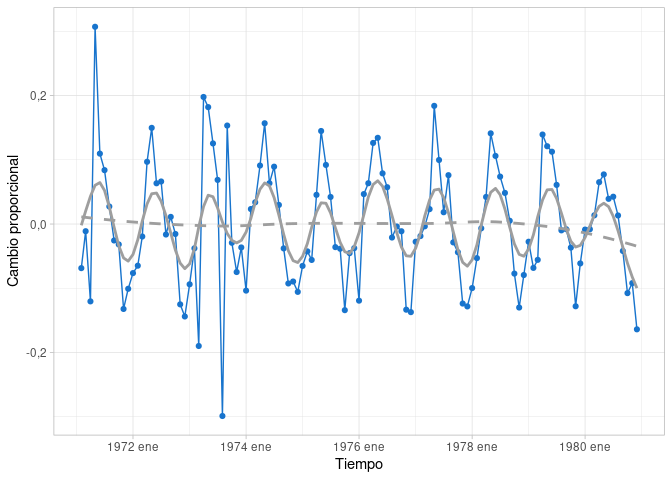
\includegraphics{/home/marcelo/MEGAsync/Msc-Math-Applied/Series Temporales/output/Lab-Session-8-FPP_files/figure-latex/transform-1} \end{center}

Como se muestra, el patrón anual persiste en la serie, y se hacen mas visibles las desviaciones que antes estaban ocultas por el componente estacional. Dos observaciones destacan como valores atípicos en la serie, al inicio del primer pico a mediados de 1971, y en el primer valle en 1973.

\hypertarget{elecciuxf3n-de-un-modelo.}{%
\subsection{Elección de un modelo.}\label{elecciuxf3n-de-un-modelo.}}

Para un primer análisis de la correlación serial de la serie, verificamos las ACF y PACF (figura \ref{fig:acf-pacf}).

\begin{Shaded}
\begin{Highlighting}[]
\NormalTok{cm_transf }\OperatorTok
\StringTok{  }\KeywordTok{ACF}\NormalTok{(prop_change, }\DataTypeTok{lag_max=}\DecValTok{50}\NormalTok{) }\OperatorTok
\StringTok{  }\KeywordTok{autoplot}\NormalTok{() }\OperatorTok{+}
\StringTok{    }\KeywordTok{theme_light}\NormalTok{() }\OperatorTok{+}
\StringTok{    }\KeywordTok{xlab}\NormalTok{(}\StringTok{"lag"}\NormalTok{) }\OperatorTok{+}\StringTok{ }
\StringTok{    }\KeywordTok{ylab}\NormalTok{(latex2exp}\OperatorTok{::}\KeywordTok{TeX}\NormalTok{(}\StringTok{"$}\CharTok{\textbackslash{}\textbackslash{}}\StringTok{rho(s, t)$"}\NormalTok{)) ->}\StringTok{ }\NormalTok{acf}

\NormalTok{cm_transf }\OperatorTok
\StringTok{  }\KeywordTok{PACF}\NormalTok{(prop_change, }\DataTypeTok{lag_max=}\DecValTok{50}\NormalTok{) }\OperatorTok
\StringTok{  }\KeywordTok{autoplot}\NormalTok{() }\OperatorTok{+}
\StringTok{    }\KeywordTok{theme_light}\NormalTok{() }\OperatorTok{+}
\StringTok{    }\KeywordTok{xlab}\NormalTok{(}\StringTok{"lag"}\NormalTok{) }\OperatorTok{+}\StringTok{ }
\StringTok{    }\KeywordTok{ylab}\NormalTok{(latex2exp}\OperatorTok{::}\KeywordTok{TeX}\NormalTok{(}\StringTok{"$}\CharTok{\textbackslash{}\textbackslash{}}\StringTok{rho(s, t)$"}\NormalTok{))->}\StringTok{ }\NormalTok{pacf}

\NormalTok{cowplot}\OperatorTok{::}\KeywordTok{plot_grid}\NormalTok{(acf, pacf, }\DataTypeTok{nrow=}\DecValTok{1}\NormalTok{)}
\end{Highlighting}
\end{Shaded}

\begin{center}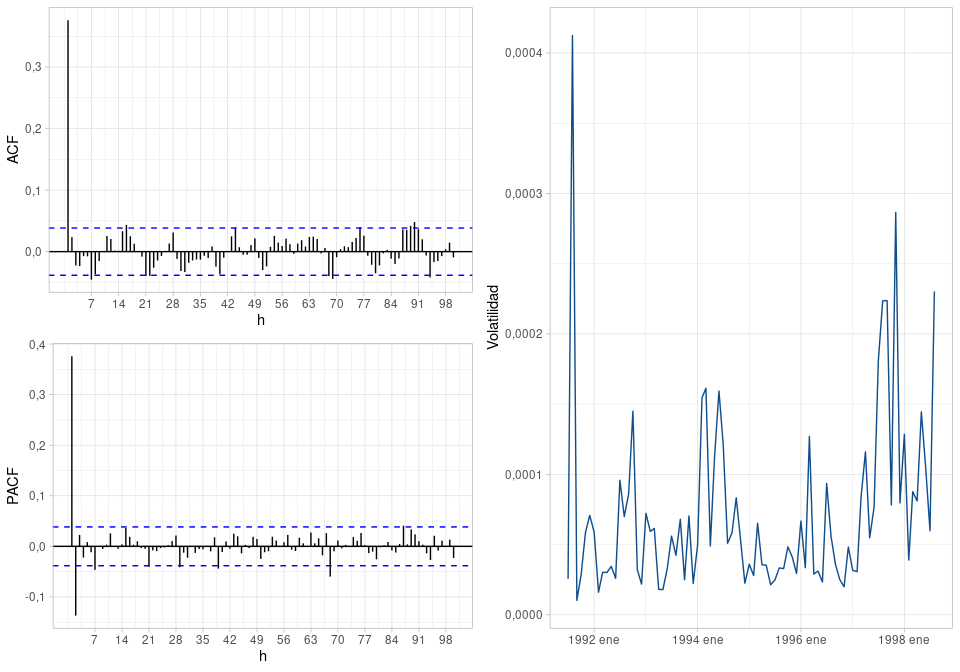
\includegraphics{/home/marcelo/MEGAsync/Msc-Math-Applied/Series Temporales/output/Lab-Session-8-FPP_files/figure-latex/acf-pacf-1} \end{center}

\begin{itemize}
\tightlist
\item
  💹 La ACF indica que seria apropiada una diferencia de orden \(D=1\) para el componente estacional, y un parámetro autoregresivo de orden \(P=1\). También se observa que el periodo debería ser \(s=6\), dado que los picos de mayor magnitud se registran en \(6k\) para \(k=1,2,\ldots\). Sin embargo, como el patrón es anual, se elige un periodo de \(s=12\) dado que en un intervalo de 12 meses se completa un ciclo en la ACF.
\item
  💹 La PACF confirma que se debería elegir \(P=1\), dada la correlación significativa en el \(h=6\), pero en más ningún múltiplo de 6.
\item
  💹 Dado que la ACF es decayente en los \emph{lags} mostrados, y que la PACF se corta en el \(h=1\), se usa un orden \(p=1\) para la parte \(ARMA\).
\item
  💹 Se observan un par de correlaciones significativas en la PACF, donde la correlación en \(h=4\) es la mas importante. La otra se encuentra en \(h=22\). Estas correlaciones aparecen significativas probablemente debido al patrón anual oscilante combinado con los cambios abruptos durante los picos y valles de la serie: en estos \emph{lags} se encuentran espaciados casi 2 años, y coinciden con la entrada a los picos y valles de la serie original.
\end{itemize}

Los resultados de la prueba de Dickey-Fuller aumentada para comprobar estacionaridad de la serie muestran que el incremento proporcional de unidades es estacionaria (\(DF_T=\text{-6,95}\), \(p=\text{0,01}\)), por lo que no es necesario una diferencia en el componente ARMA.

Se ajusta entonces un modelo \(ARIMA(1, 0, 0)(0, 1, 1)_{12}\), y se compara con un modelo \(ARIMA(2, 0, 2)(0, 1, 1)_{12}\) estimado minimizando la sumatoria de cuadrados condicional, encontrado por medio de una búsqueda del mejor modelo en el espacio de parámetros (mejor en el sentido de sumatoria de cuadrados mínima).

Se escribe el modelo inferido de los descriptivos:

\[
\begin{aligned}
  \Delta_{12}\phi(B)r_t = \Theta(B) w_t  & \Rightarrow \\
    & \Rightarrow (1 - B^12)(1 - \phi B) r_t = (1 - \Theta B) w_t \\
\end{aligned}
\]

el cual se expande como:

\[r_t = \phi r_{t-1} + r_{t-12} + \phi r_{t-13} + w_t + \Theta w_{t-1}\label{eq:model}\]

\hypertarget{estaduxedsticos-de-bondad-de-ajuste.}{%
\subsubsection{Estadísticos de Bondad de Ajuste.}\label{estaduxedsticos-de-bondad-de-ajuste.}}

Los resultados de los ajustes se muestran en la tabla \ref{tab:fitting-sarima}, los cuales indican que el modelo dado en la ecuación \ref{eq:model} no difiere demasiado del modelo encontrado al tantear el espacio de parámetros, en términos de robustez y precisión, dada la varianza residual, \(RMSE\) y \(MAE\) similares.

Además, el modelo \(ARIMA(2, 0, 2)(0, 1, 1)_{12}\) parece ser preferible según los valores obtenidos en términos de la información proveída por el modelo (\(AIC\), \(AICc\) y \(BIC\)). Esto se debe (dada la similitud de varianzas residuales), solo al aumento en la penalización consecuencia de la mayor cantidad de parámetros estimados en el modelo \(ARIMA(2, 0, 2)(0, 1, 1)_{12}\).

\begin{Shaded}
\begin{Highlighting}[]
\NormalTok{.model <-}\StringTok{ }\KeywordTok{c}\NormalTok{(}\StringTok{"$ARIMA(1,0,0)(0,1,1)_12$"}\NormalTok{, }\StringTok{"ARIMA(2,0,2)(0,1,1)_12"}\NormalTok{)}

\NormalTok{information_based }\OperatorTok
\StringTok{  }\KeywordTok{left_join}\NormalTok{(error_based) }\OperatorTok
\StringTok{  }\KeywordTok{select}\NormalTok{(sigma2}\OperatorTok{:}\NormalTok{BIC, ME}\OperatorTok{:}\NormalTok{MAE) }\OperatorTok
\StringTok{  }\NormalTok{tibble}\OperatorTok{::}\KeywordTok{add_column}\NormalTok{(}\DataTypeTok{.model=}\NormalTok{.model, }\DataTypeTok{.before=}\DecValTok{1}\NormalTok{) }\OperatorTok
\StringTok{  }\NormalTok{knitr}\OperatorTok{::}\KeywordTok{kable}\NormalTok{(}\DataTypeTok{digits=}\KeywordTok{c}\NormalTok{(}\OtherTok{NA}\NormalTok{, }\DecValTok{4}\NormalTok{, }\DecValTok{2}\NormalTok{, }\DecValTok{1}\NormalTok{, }\DecValTok{1}\NormalTok{, }\DecValTok{1}\NormalTok{, }\DecValTok{4}\NormalTok{, }\DecValTok{4}\NormalTok{, }\DecValTok{4}\NormalTok{), }
    \DataTypeTok{align=}\StringTok{'lcccccccccc'}\NormalTok{, }\DataTypeTok{escape=}\OtherTok{FALSE}\NormalTok{,}
    \DataTypeTok{col.names=}\KeywordTok{c}\NormalTok{(}\StringTok{"Modelo"}\NormalTok{, }\StringTok{"$}\CharTok{\textbackslash{}\textbackslash{}}\StringTok{sigma^2$"}\NormalTok{, }\StringTok{"Func. Verosim."}\NormalTok{, }\StringTok{"AIC"}\NormalTok{, }\StringTok{"AICc"}\NormalTok{, }\StringTok{"BIC"}\NormalTok{, }\StringTok{"ME"}\NormalTok{, }\StringTok{"RMSE"}\NormalTok{, }\StringTok{"MAE"}\NormalTok{),}
    \DataTypeTok{caption=}\StringTok{"Estadísticos de bondad de ajuste de los modelos SARIMA ajustados."}\NormalTok{)}
\end{Highlighting}
\end{Shaded}

\begin{table}

\caption{\label{tab:fitting-sarima}Estadísticos de bondad de ajuste de los modelos SARIMA ajustados.}
\centering
\begin{tabular}[t]{l|c|c|c|c|c|c|c|c}
\hline
Modelo & $\sigma^2$ & Func. Verosim. & AIC & AICc & BIC & ME & RMSE & MAE\\
\hline
$ARIMA(1,0,0)(0,1,1)_12$ & 0,0034 & 143,79 & -281,6 & -281,4 & -273,6 & 0,0005 & 0,0547 & 0,0372\\
\hline
ARIMA(2,0,2)(0,1,1)_12 & 0,0033 & 148,93 & -285,9 & -285,0 & -269,8 & 0,0007 & 0,0531 & 0,0376\\
\hline
\end{tabular}
\end{table}

\hypertarget{gruxe1ficos-diagnuxf3sticos-de-residuales.}{%
\subsubsection{Gráficos diagnósticos de residuales.}\label{gruxe1ficos-diagnuxf3sticos-de-residuales.}}

Al verificar el comportamiento de los residuales para el modelo candidato, \(ARIMA(1,0,0)(0,1,1)_{12}\), se obtiene que los residuales no parecen estar correlacionados entre si, evaluando con respecto al retraso 12, aunque el valor de probabilidad obtenido es apenas marginal (\(Q=\text{15,289}\), \(p=\text{0,0537708}\)).
En el gráfico para ACF y PACF se muestra un pico de correlación significativa con respeto al \emph{lag} 5, lo cual indica la falta de un retraso en el modelo considerado.

\begin{Shaded}
\begin{Highlighting}[]
\NormalTok{augmented_data }\OperatorTok
\StringTok{  }\KeywordTok{ACF}\NormalTok{(.innov, }\DataTypeTok{lag_max=}\DecValTok{50}\NormalTok{) }\OperatorTok
\StringTok{  }\KeywordTok{autoplot}\NormalTok{() }\OperatorTok{+}
\StringTok{    }\KeywordTok{theme_light}\NormalTok{() }\OperatorTok{+}
\StringTok{    }\KeywordTok{xlab}\NormalTok{(}\StringTok{"lag"}\NormalTok{) }\OperatorTok{+}\StringTok{ }
\StringTok{    }\KeywordTok{ylab}\NormalTok{(latex2exp}\OperatorTok{::}\KeywordTok{TeX}\NormalTok{(}\StringTok{"$}\CharTok{\textbackslash{}\textbackslash{}}\StringTok{rho(s, t)$"}\NormalTok{)) ->}\StringTok{ }\NormalTok{acf}

\NormalTok{augmented_data }\OperatorTok
\StringTok{  }\KeywordTok{PACF}\NormalTok{(.innov, }\DataTypeTok{lag_max=}\DecValTok{50}\NormalTok{) }\OperatorTok
\StringTok{  }\KeywordTok{autoplot}\NormalTok{() }\OperatorTok{+}
\StringTok{    }\KeywordTok{theme_light}\NormalTok{() }\OperatorTok{+}
\StringTok{    }\KeywordTok{xlab}\NormalTok{(}\StringTok{"lag"}\NormalTok{) }\OperatorTok{+}\StringTok{ }
\StringTok{    }\KeywordTok{ylab}\NormalTok{(latex2exp}\OperatorTok{::}\KeywordTok{TeX}\NormalTok{(}\StringTok{"$}\CharTok{\textbackslash{}\textbackslash{}}\StringTok{rho(s, t)$"}\NormalTok{))->}\StringTok{ }\NormalTok{pacf }

\NormalTok{res_series <-}\StringTok{ }\NormalTok{augmented_data }\OperatorTok
\StringTok{  }\KeywordTok{autoplot}\NormalTok{(.std.resid, }\DataTypeTok{colour=}\StringTok{"orange"}\NormalTok{) }\OperatorTok{+}
\StringTok{  }\KeywordTok{geom_point}\NormalTok{(}\KeywordTok{aes}\NormalTok{(}\DataTypeTok{y=}\NormalTok{.std.resid), }\DataTypeTok{colour=}\StringTok{"orange"}\NormalTok{) }\OperatorTok{+}
\StringTok{  }\KeywordTok{scale_x_yearmonth}\NormalTok{(}\DataTypeTok{date_labels =} \StringTok{"%Y"}\NormalTok{) }\OperatorTok{+}
\StringTok{  }\KeywordTok{xlab}\NormalTok{(}\StringTok{"Tiempo"}\NormalTok{) }\OperatorTok{+}
\StringTok{  }\KeywordTok{ylab}\NormalTok{(}\StringTok{"Residuales Estandarizados"}\NormalTok{) }\OperatorTok{+}\StringTok{ }
\StringTok{  }\KeywordTok{geom_hline}\NormalTok{(}\DataTypeTok{yintercept=}\KeywordTok{c}\NormalTok{(}\DecValTok{0}\NormalTok{, }\FloatTok{1.96}\NormalTok{, }\FloatTok{-1.96}\NormalTok{), }
    \DataTypeTok{color=}\KeywordTok{c}\NormalTok{(}\StringTok{"black"}\NormalTok{, }\DecValTok{200}\NormalTok{, }\DecValTok{200}\NormalTok{), }\DataTypeTok{linetype=}\KeywordTok{c}\NormalTok{(}\DecValTok{1}\NormalTok{, }\DecValTok{2}\NormalTok{, }\DecValTok{2}\NormalTok{)) }\OperatorTok{+}
\StringTok{  }\KeywordTok{theme_light}\NormalTok{() }

\NormalTok{res_qq_plot <-}\StringTok{ }\NormalTok{augmented_data }\OperatorTok\StringTok{ }
\StringTok{  }\KeywordTok{ggplot}\NormalTok{(}\KeywordTok{aes}\NormalTok{(}\DataTypeTok{sample =}\NormalTok{ .resid)) }\OperatorTok{+}\StringTok{ }
\StringTok{  }\KeywordTok{stat_qq}\NormalTok{() }\OperatorTok{+}\StringTok{ }\KeywordTok{stat_qq_line}\NormalTok{(}\DataTypeTok{color=}\StringTok{"red"}\NormalTok{) }\OperatorTok{+}\StringTok{ }
\StringTok{  }\KeywordTok{theme_light}\NormalTok{()}

\NormalTok{cowplot}\OperatorTok{::}\KeywordTok{plot_grid}\NormalTok{(acf, pacf, res_series, res_qq_plot, }
  \DataTypeTok{nrow=}\DecValTok{1}\NormalTok{, }\DataTypeTok{align=}\StringTok{"h"}\NormalTok{,}
  \DataTypeTok{labels=}\KeywordTok{c}\NormalTok{(}\StringTok{"a)"}\NormalTok{, }\StringTok{"b)"}\NormalTok{, }\StringTok{"c)"}\NormalTok{, }\StringTok{"d)"}\NormalTok{), }
  \DataTypeTok{label_size=}\DecValTok{11}\NormalTok{, }
  \DataTypeTok{label_fontface=}\StringTok{"italic"}\NormalTok{)}
\end{Highlighting}
\end{Shaded}

\begin{center}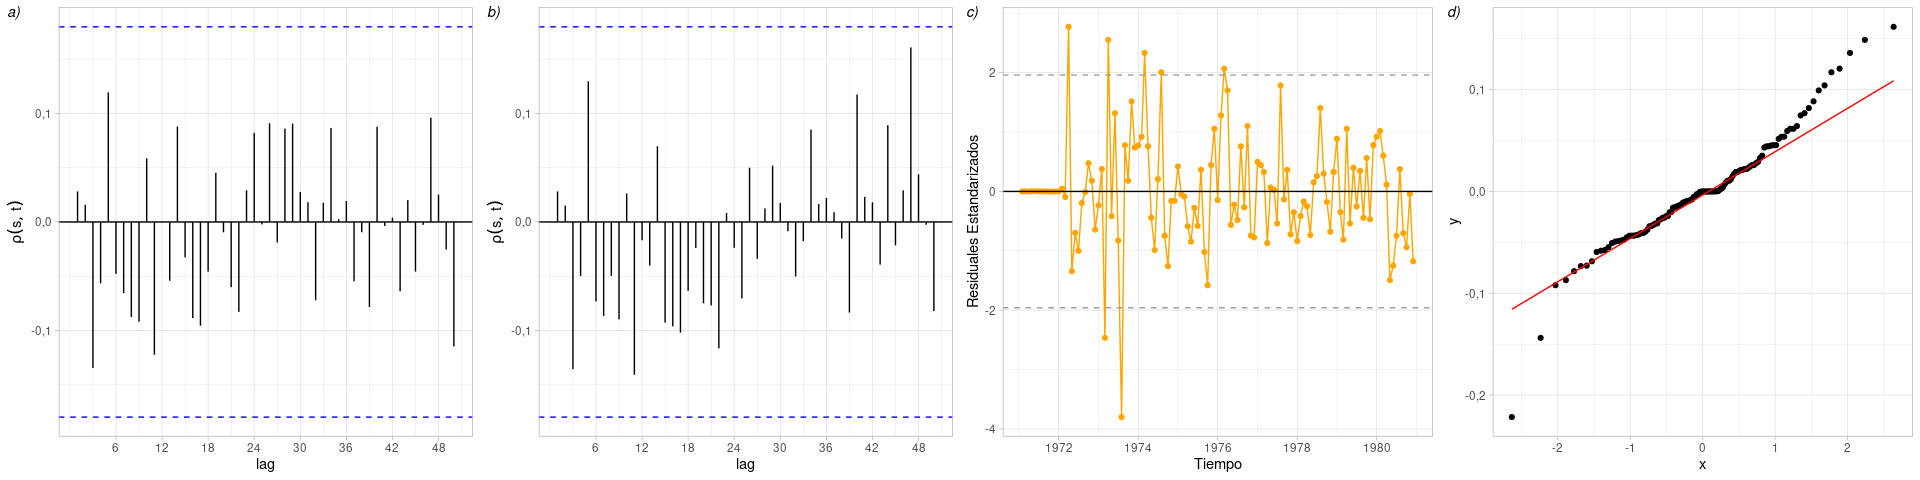
\includegraphics{/home/marcelo/MEGAsync/Msc-Math-Applied/Series Temporales/output/Lab-Session-8-FPP_files/figure-latex/diagnostics-plots-1} \end{center}

Más aun, el gráfico de residuales estandarizados y el gráfico \emph{QQ} muestran claramente que los residuales no son normales.
Se observa un patrón no aleatorio de distribución de los residuales alrededor de la media (secciones donde las observaciones caen mucho por encima de la media, y secciones donde caen por debajo). Además, se pueden notar observaciones atípicas, 8 de ellas específicamente, como se muestra en la tabla @ref\{tab:outliers\}.
Se puede notar claramente que 3 de ellas caen en 1973, donde el comportamiento de la serie es anormal comparado con los otros años, y el resto corresponden a puntos de entrada a los picos y a los picos observados luego de 1973.

\begin{Shaded}
\begin{Highlighting}[]
\NormalTok{augmented_data }\OperatorTok
\StringTok{  }\KeywordTok{filter}\NormalTok{(}
\NormalTok{    .resid }\OperatorTok{<}\StringTok{ }\KeywordTok{quantile}\NormalTok{(.resid, }\FloatTok{0.25}\NormalTok{) }\OperatorTok{-}\StringTok{ }\FloatTok{1.5} \OperatorTok{*}\StringTok{ }\KeywordTok{IQR}\NormalTok{(.resid) }\OperatorTok{|}
\StringTok{    }\NormalTok{.resid }\OperatorTok{>}\StringTok{ }\KeywordTok{quantile}\NormalTok{(.resid, }\FloatTok{0.75}\NormalTok{) }\OperatorTok{+}\StringTok{ }\FloatTok{1.5} \OperatorTok{*}\StringTok{ }\KeywordTok{IQR}\NormalTok{(.resid)}
\NormalTok{  ) }\OperatorTok
\StringTok{  }\KeywordTok{select}\NormalTok{(}\OperatorTok{-}\NormalTok{.resid, }\OperatorTok{-}\NormalTok{.model) }\OperatorTok
\StringTok{  }\NormalTok{knitr}\OperatorTok{::}\KeywordTok{kable}\NormalTok{(}\DataTypeTok{digits=}\KeywordTok{c}\NormalTok{(}\DecValTok{0}\NormalTok{, }\DecValTok{4}\NormalTok{, }\DecValTok{4}\NormalTok{, }\DecValTok{3}\NormalTok{, }\DecValTok{3}\NormalTok{, }\DecValTok{2}\NormalTok{),}
    \DataTypeTok{escape=}\OtherTok{FALSE}\NormalTok{, }\DataTypeTok{align=}\StringTok{'lcccccc'}\NormalTok{,}
    \DataTypeTok{col.names=}\KeywordTok{c}\NormalTok{(}\StringTok{"Año"}\NormalTok{, }\StringTok{"$r_t$"}\NormalTok{, }\StringTok{"Predicho"}\NormalTok{, }\StringTok{"Residuo"}\NormalTok{, }\StringTok{"Res. Estand."}\NormalTok{),}
    \DataTypeTok{caption=}\StringTok{"Observaciones atípicas registradas para los cambios proporcionales en el número de unidades en inventario de leche condensada."}\NormalTok{)}
\end{Highlighting}
\end{Shaded}

\begin{table}

\caption{\label{tab:outliers}Observaciones atípicas registradas para los cambios proporcionales en el número de unidades en inventario de leche condensada.}
\centering
\begin{tabular}[t]{l|c|c|c|c}
\hline
Año & $r_t$ & Predicho & Residuo & Res. Estand.\\
\hline
1972 abr & 0,0969 & -0,0623 & 0,159 & 2,735\\
\hline
1973 mar & -0,1899 & -0,0469 & -0,143 & -2,457\\
\hline
1973 abr & 0,1979 & 0,0543 & 0,144 & 2,467\\
\hline
1973 ago & -0,2990 & -0,0383 & -0,261 & -4,477\\
\hline
1974 mar & 0,0338 & -0,0807 & 0,115 & 1,967\\
\hline
1974 ago & 0,0297 & -0,0885 & 0,118 & 2,032\\
\hline
1976 mar & 0,0635 & -0,0613 & 0,125 & 2,145\\
\hline
1977 ago & 0,0761 & -0,0359 & 0,112 & 1,924\\
\hline
\end{tabular}
\end{table}

Todo lo mencionado, parece indicar que aun existe una estructura de dependencia dentro de la serie que no se ha especificado, y que se debe optar por un modelo distinto. Los resultados parecen indicar que se debe considerar un modelo con el quinto \emph{lag} como regresor.

\hypertarget{anuxe1lisis-de-correlaciones-de-r_t-y-r_t-h.}{%
\subsubsection{\texorpdfstring{Análisis de correlaciones de \(r_t\) y \(r_{t-h}\).}{Análisis de correlaciones de r\_t y r\_\{t-h\}.}}\label{anuxe1lisis-de-correlaciones-de-r_t-y-r_t-h.}}

Dado los resultados encontrados para el primer modelo ajustado, se decide hacer un análisis de correlación entre la serie temporal con respecto a las series temporales retrasadas (figura \ref{fig:bivariate-lag}).

\begin{Shaded}
\begin{Highlighting}[]
\NormalTok{tscleaned }\OperatorTok
\StringTok{  }\KeywordTok{gg_lag}\NormalTok{(prop_change, }\DataTypeTok{period=}\DecValTok{12}\NormalTok{, }\DataTypeTok{lags=}\DecValTok{1}\OperatorTok{:}\DecValTok{12}\NormalTok{, }\DataTypeTok{geom=}\StringTok{"point"}\NormalTok{) }\OperatorTok{+}
\StringTok{  }\KeywordTok{theme_light}\NormalTok{() }\OperatorTok{+}
\StringTok{  }\KeywordTok{theme}\NormalTok{(}\DataTypeTok{legend.position=}\StringTok{"none"}\NormalTok{) }\OperatorTok{+}
\StringTok{  }\KeywordTok{facet_wrap}\NormalTok{(}\OperatorTok{~}\NormalTok{.lag, }
    \DataTypeTok{labeller=}\KeywordTok{as_labeller}\NormalTok{(}\KeywordTok{setNames}\NormalTok{(}\KeywordTok{paste}\NormalTok{(}\StringTok{"h ="}\NormalTok{, }\DecValTok{1}\OperatorTok{:}\DecValTok{12}\NormalTok{), }\KeywordTok{paste}\NormalTok{(}\StringTok{"lag"}\NormalTok{, }\DecValTok{1}\OperatorTok{:}\DecValTok{12}\NormalTok{)))) }\OperatorTok{+}
\StringTok{  }\KeywordTok{xlab}\NormalTok{(}\StringTok{'lag(Cambio proporcional, h)'}\NormalTok{) }\OperatorTok{+}\StringTok{ }
\StringTok{  }\KeywordTok{ylab}\NormalTok{(}\StringTok{'Cambio proporcional'}\NormalTok{)}
\end{Highlighting}
\end{Shaded}

\begin{center}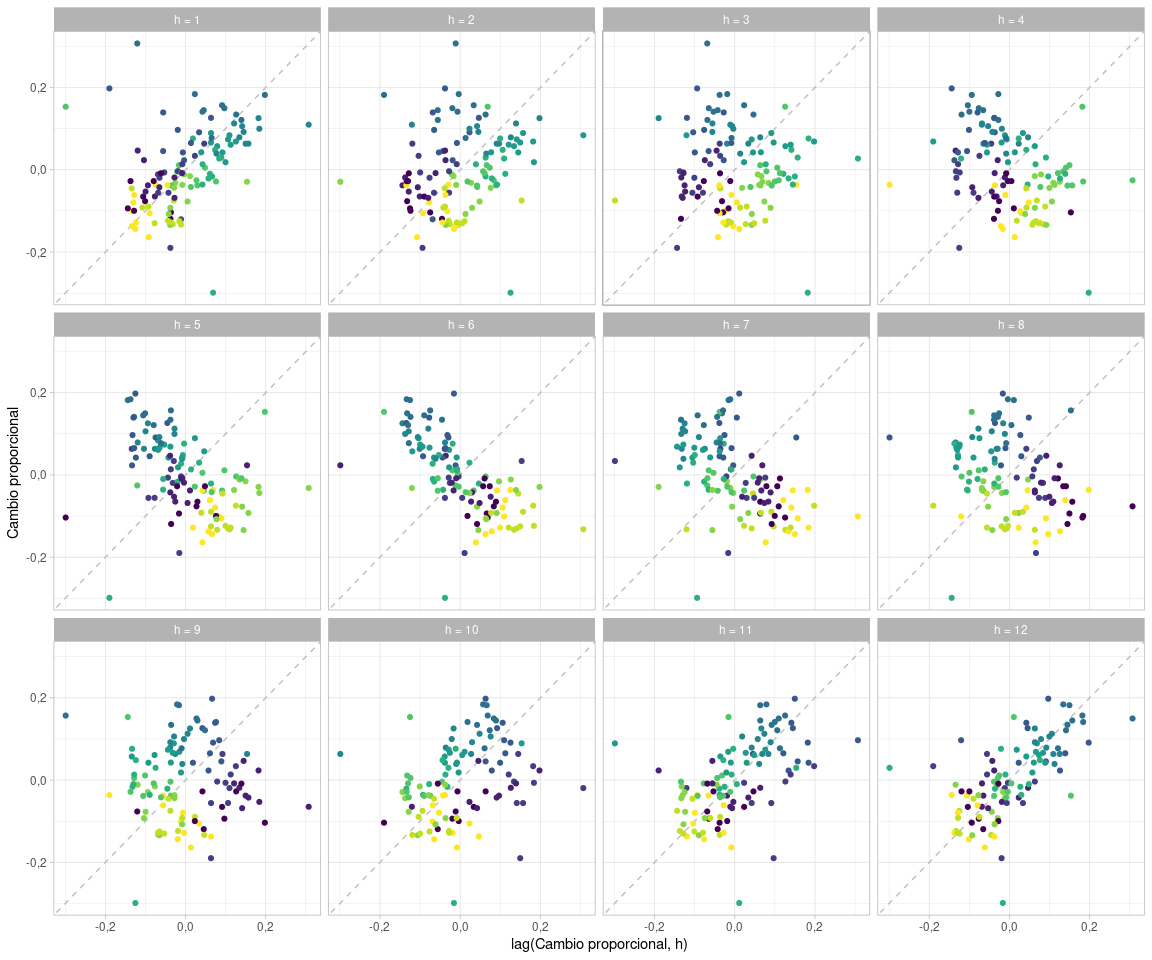
\includegraphics{/home/marcelo/MEGAsync/Msc-Math-Applied/Series Temporales/output/Lab-Session-8-FPP_files/figure-latex/bivariate-lag-1} \end{center}

La dependencia de la serie en \(t\) con respecto a los valores en \(t-1\) se toma en cuenta dentro del modelo ajustado antes, al considerar un modelo autoregresivo de orden \(p=1\), al igual que la correlación positiva con respecto al 12vo retraso.
La correlación con \(h=3\) no es significativa, y en \(h=2\) y \(h=4\) las correlaciones son pequeñas, comparadas con las correlaciones observadas en \(h=5\) y \(h=6\) (las cuales son negativas y más importantes), y que parecen ser no lineales para valores mayores a \(0{,}05\).

Para estas variables retrasadas, la correlación negativa puede modelarse de dos formas: \emph{i)} considerando un solo modelo con regresores \(r_{t-5}\) y \(r_{t-5}^2\), dada la curvatura y forma no lineal de la serie; o \emph{ii)} generando un modelo a trozos con un regresor lineal \(r_{t-6}\), cuyo coeficiente asociado cambia dependiendo de si \(r_t\) es mayor a \(0{,}05\).

\hypertarget{regresiuxf3n-con-variables-retrasadas.}{%
\subsection{Regresión con variables retrasadas.}\label{regresiuxf3n-con-variables-retrasadas.}}

Se busca modelar, en el primer caso, un modelo de la forma:

\[
r_t = \phi r_{t-1} + \phi r_{t-12} + \phi r_{t-13} + \beta_1 r_{t-5} + \beta_2 r_{t-5}^2 + w_t + \Theta w_{t-1}
(\\#eq:model-reg)
\]

donde \(\beta_1\) y \(\beta_2\) son los coeficientes de regresión. En el segundo caso, se necesita de una variable \emph{dummy} \(D_{t-5}\) la cual es 0 si \(r_{t-6} < 0{,}05\) y 1 de otra forma, generando el modelo a trozos:

\[
r_t = \begin{cases}
  \omega + \beta_1 r_{t-5} &  r_{t-5} < 0{,}05 \\
  \omega + \beta_2 + (\beta_1 + \beta_3) r_{t-5} & r_{t-5} \ge 0{,}05
\end{cases}
 \label{eq:model-reg-trozos}
\]

donde \(\omega = \phi r_{t-1} + \phi r_{t-12} + \phi r_{t-13} + w_t + \Theta w_{t-1}\) es el componente ARIMA y, de nuevo, \(\beta_1\) y \(\beta_2\) son los coeficientes de regresión para \(r_{t-5}\) y \(D_{t-5}\), y \(\beta_3\) es el coeficiente de la interacción \(D_{t-5}r_{t-5}\).

\hypertarget{estaduxedsticos-de-bondad-de-ajuste.-1}{%
\subsubsection{Estadísticos de Bondad de Ajuste.}\label{estaduxedsticos-de-bondad-de-ajuste.-1}}

\begin{Shaded}
\begin{Highlighting}[]
\NormalTok{models_xreg <-}\StringTok{ }\KeywordTok{c}\NormalTok{(.model, }
  \StringTok{"$ARIMA(1,0,0)(0,1,1)_12 }\CharTok{\textbackslash{}\textbackslash{}}\StringTok{text\{ (no lineal con \}r_\{t-5\}^2}\CharTok{\textbackslash{}\textbackslash{}}\StringTok{text\{)\}$"}\NormalTok{, }
  \StringTok{"$ARIMA(1,0,0)(0,1,1)_6 }\CharTok{\textbackslash{}\textbackslash{}}\StringTok{text\{ (a trozos)\}$"}\NormalTok{)}

\NormalTok{information_based_}\DecValTok{2} \OperatorTok
\StringTok{  }\KeywordTok{left_join}\NormalTok{(error_based_}\DecValTok{2}\NormalTok{) }\OperatorTok
\StringTok{  }\KeywordTok{select}\NormalTok{(sigma2}\OperatorTok{:}\NormalTok{BIC, ME}\OperatorTok{:}\NormalTok{MAE) }\OperatorTok
\StringTok{  }\NormalTok{tibble}\OperatorTok{::}\KeywordTok{add_column}\NormalTok{(}\DataTypeTok{model=}\NormalTok{models_xreg, }\DataTypeTok{.before=}\DecValTok{1}\NormalTok{) }\OperatorTok
\StringTok{  }\NormalTok{knitr}\OperatorTok{::}\KeywordTok{kable}\NormalTok{(}\DataTypeTok{digits=}\KeywordTok{c}\NormalTok{(}\OtherTok{NA}\NormalTok{, }\DecValTok{4}\NormalTok{, }\DecValTok{2}\NormalTok{, }\DecValTok{1}\NormalTok{, }\DecValTok{1}\NormalTok{, }\DecValTok{1}\NormalTok{, }\DecValTok{4}\NormalTok{, }\DecValTok{4}\NormalTok{, }\DecValTok{4}\NormalTok{), }
    \DataTypeTok{align=}\StringTok{'lcccccccccc'}\NormalTok{, }\DataTypeTok{escape=}\OtherTok{FALSE}\NormalTok{,}
    \DataTypeTok{col.names=}\KeywordTok{c}\NormalTok{(}\StringTok{"Modelo"}\NormalTok{, }\StringTok{"$}\CharTok{\textbackslash{}\textbackslash{}}\StringTok{sigma^2$"}\NormalTok{, }\StringTok{"Func. Verosim."}\NormalTok{, }\StringTok{"AIC"}\NormalTok{, }\StringTok{"AICc"}\NormalTok{, }\StringTok{"BIC"}\NormalTok{, }\StringTok{"ME"}\NormalTok{, }\StringTok{"RMSE"}\NormalTok{, }\StringTok{"MAE"}\NormalTok{),}
    \DataTypeTok{caption=}\StringTok{"Estadísticos de bondad de ajuste de los modelos SARIMA ajustados."}\NormalTok{)}
\end{Highlighting}
\end{Shaded}

\begin{table}

\caption{\label{tab:lagged-regression}Estadísticos de bondad de ajuste de los modelos SARIMA ajustados.}
\centering
\begin{tabular}[t]{l|c|c|c|c|c|c|c|c}
\hline
Modelo & $\sigma^2$ & Func. Verosim. & AIC & AICc & BIC & ME & RMSE & MAE\\
\hline
$ARIMA(1,0,0)(0,1,1)_12$ & 0,0033 & 148,93 & -285,9 & -285,0 & -269,8 & 0,0007 & 0,0531 & 0,0376\\
\hline
ARIMA(2,0,2)(0,1,1)_12 & 0,0026 & 147,67 & -285,3 & -284,7 & -272,2 & -0,0002 & 0,0471 & 0,0339\\
\hline
$ARIMA(1,0,0)(0,1,1)_12 \text{ (no lineal con }r_{t-5}^2\text{)}$ & 0,0026 & 148,38 & -284,8 & -283,9 & -269,0 & 0,0006 & 0,0468 & 0,0336\\
\hline
$ARIMA(1,0,0)(0,1,1)_6 \text{ (a trozos)}$ & 0,0034 & 143,79 & -281,6 & -281,4 & -273,6 & 0,0005 & 0,0547 & 0,0372\\
\hline
\end{tabular}
\end{table}

Los estadístico de bondad de ajuste muestran que las varianzas residuales de los modelos mostrados en las ecuaciones \eqref{eq:model-reg} y \eqref{eq:model-reg-trozos} son menores a la varianza residual del modelo \(ARIMA(1,0,0)(0,1,1)_6\) sin regresores.
De igual forma, las demás medidas basadas en residuales RMSE, MAE y ME, no varían demasiado con respecto a los encontrados para el primer modelo ajustado, pero son, claro, menores.
Por otro lado, los valores de AIC y BIC para el modelo de regresión a trozos y el que usa una dependencia cuadrática son menores que los del primer modelo ajustado anteriormente (sin regresores).

\hypertarget{gruxe1ficos-diagnuxf3sticos-de-residuales.-1}{%
\subsubsection{Gráficos diagnósticos de residuales.}\label{gruxe1ficos-diagnuxf3sticos-de-residuales.-1}}

Los gráficos de residuales se muestran en la figura \ref{fig:diagnostics-plots-2} para el modelo de la ecuación \eqref{eq:model-reg}, con la dependencia cuadrática (el cual se selecciona al revisar los residuales).
Se puede observar que ya no existen correlaciones significativas, aunque se observa, principalmente en el PACF, que hay una cantidad inusualmente grande de correlaciones negativas en una sección en la primera mitad del gráfico.

\begin{Shaded}
\begin{Highlighting}[]
\NormalTok{augmented_data_}\DecValTok{2} \OperatorTok
\StringTok{  }\KeywordTok{ACF}\NormalTok{(.innov, }\DataTypeTok{lag_max=}\DecValTok{50}\NormalTok{) }\OperatorTok
\StringTok{  }\KeywordTok{autoplot}\NormalTok{() }\OperatorTok{+}
\StringTok{    }\KeywordTok{theme_light}\NormalTok{() }\OperatorTok{+}
\StringTok{    }\KeywordTok{xlab}\NormalTok{(}\StringTok{"lag"}\NormalTok{) }\OperatorTok{+}\StringTok{ }
\StringTok{    }\KeywordTok{ylab}\NormalTok{(latex2exp}\OperatorTok{::}\KeywordTok{TeX}\NormalTok{(}\StringTok{"$}\CharTok{\textbackslash{}\textbackslash{}}\StringTok{rho(s, t)$"}\NormalTok{)) ->}\StringTok{ }\NormalTok{acf}

\NormalTok{augmented_data_}\DecValTok{2} \OperatorTok
\StringTok{  }\KeywordTok{PACF}\NormalTok{(.innov, }\DataTypeTok{lag_max=}\DecValTok{50}\NormalTok{) }\OperatorTok
\StringTok{  }\KeywordTok{autoplot}\NormalTok{() }\OperatorTok{+}
\StringTok{    }\KeywordTok{theme_light}\NormalTok{() }\OperatorTok{+}
\StringTok{    }\KeywordTok{xlab}\NormalTok{(}\StringTok{"lag"}\NormalTok{) }\OperatorTok{+}\StringTok{ }
\StringTok{    }\KeywordTok{ylab}\NormalTok{(latex2exp}\OperatorTok{::}\KeywordTok{TeX}\NormalTok{(}\StringTok{"$}\CharTok{\textbackslash{}\textbackslash{}}\StringTok{rho(s, t)$"}\NormalTok{))->}\StringTok{ }\NormalTok{pacf }

\NormalTok{res_series <-}\StringTok{ }\NormalTok{augmented_data_}\DecValTok{2} \OperatorTok
\StringTok{  }\KeywordTok{autoplot}\NormalTok{(.std.resid, }\DataTypeTok{colour=}\StringTok{"orange"}\NormalTok{) }\OperatorTok{+}
\StringTok{  }\KeywordTok{geom_point}\NormalTok{(}\KeywordTok{aes}\NormalTok{(}\DataTypeTok{y=}\NormalTok{.std.resid), }\DataTypeTok{colour=}\StringTok{"orange"}\NormalTok{) }\OperatorTok{+}
\StringTok{  }\KeywordTok{scale_x_yearmonth}\NormalTok{(}\DataTypeTok{date_labels =} \StringTok{"%Y"}\NormalTok{) }\OperatorTok{+}
\StringTok{  }\KeywordTok{xlab}\NormalTok{(}\StringTok{"Tiempo"}\NormalTok{) }\OperatorTok{+}
\StringTok{  }\KeywordTok{ylab}\NormalTok{(}\StringTok{"Residuales Estandarizados"}\NormalTok{) }\OperatorTok{+}\StringTok{ }
\StringTok{  }\KeywordTok{geom_hline}\NormalTok{(}\DataTypeTok{yintercept=}\KeywordTok{c}\NormalTok{(}\DecValTok{0}\NormalTok{, }\FloatTok{1.96}\NormalTok{, }\FloatTok{-1.96}\NormalTok{), }
    \DataTypeTok{color=}\KeywordTok{c}\NormalTok{(}\StringTok{"black"}\NormalTok{, }\DecValTok{200}\NormalTok{, }\DecValTok{200}\NormalTok{), }\DataTypeTok{linetype=}\KeywordTok{c}\NormalTok{(}\DecValTok{1}\NormalTok{, }\DecValTok{2}\NormalTok{, }\DecValTok{2}\NormalTok{)) }\OperatorTok{+}
\StringTok{  }\KeywordTok{theme_light}\NormalTok{() }

\NormalTok{res_qq_plot <-}\StringTok{ }\NormalTok{augmented_data_}\DecValTok{2} \OperatorTok\StringTok{ }
\StringTok{  }\KeywordTok{ggplot}\NormalTok{(}\KeywordTok{aes}\NormalTok{(}\DataTypeTok{sample =}\NormalTok{ .resid)) }\OperatorTok{+}\StringTok{ }
\StringTok{  }\KeywordTok{stat_qq}\NormalTok{() }\OperatorTok{+}\StringTok{ }\KeywordTok{stat_qq_line}\NormalTok{(}\DataTypeTok{color=}\StringTok{"red"}\NormalTok{) }\OperatorTok{+}\StringTok{ }
\StringTok{  }\KeywordTok{theme_light}\NormalTok{()}

\NormalTok{cowplot}\OperatorTok{::}\KeywordTok{plot_grid}\NormalTok{(acf, pacf, res_series, res_qq_plot, }
  \DataTypeTok{nrow=}\DecValTok{1}\NormalTok{, }\DataTypeTok{align=}\StringTok{"h"}\NormalTok{,}
  \DataTypeTok{labels=}\KeywordTok{c}\NormalTok{(}\StringTok{"a)"}\NormalTok{, }\StringTok{"b)"}\NormalTok{, }\StringTok{"c)"}\NormalTok{, }\StringTok{"d)"}\NormalTok{), }
  \DataTypeTok{label_size=}\DecValTok{11}\NormalTok{, }
  \DataTypeTok{label_fontface=}\StringTok{"italic"}\NormalTok{)}
\end{Highlighting}
\end{Shaded}

\begin{center}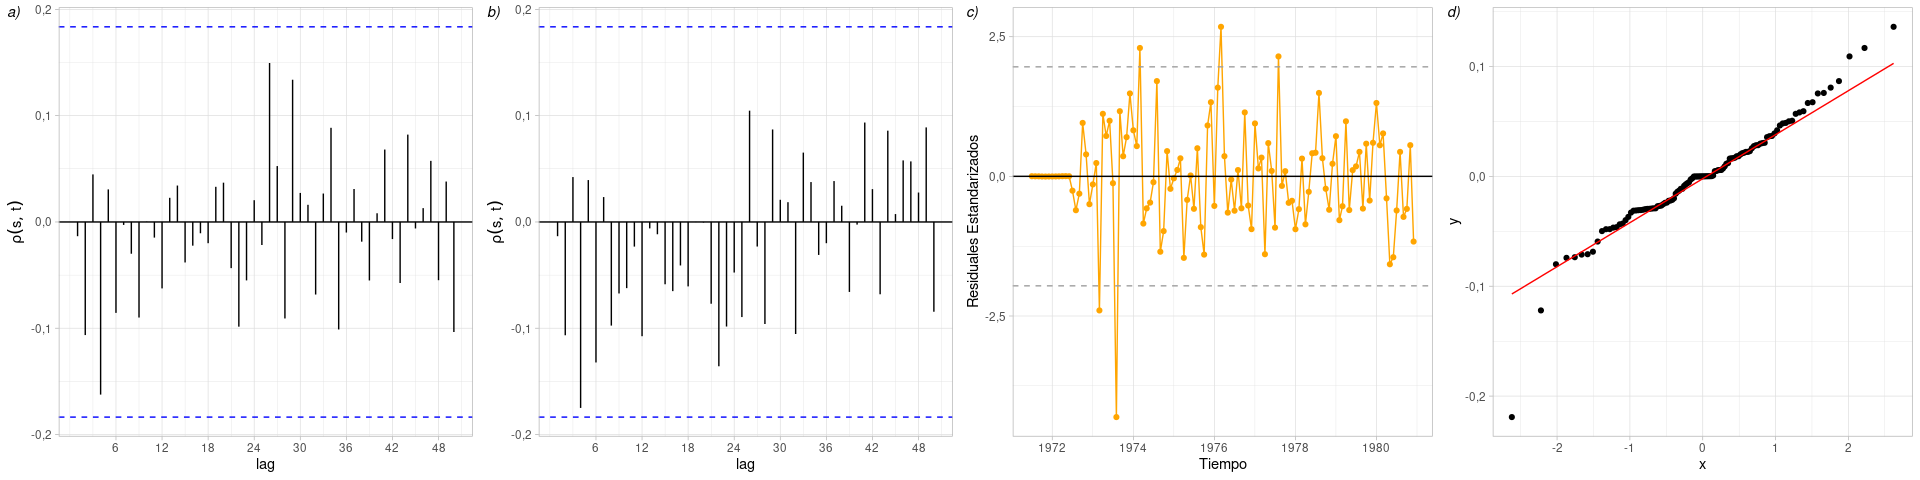
\includegraphics{/home/marcelo/MEGAsync/Msc-Math-Applied/Series Temporales/output/Lab-Session-8-FPP_files/figure-latex/diagnostics-plots-2-1} \end{center}

Por otro lado, el gráfico \emph{QQ} muestra una mejora significativa en el comportamiento de los residuales, comparado con el modelo anterior. La distribución de estos alrededor de la media se percibe mas aleatoria, y a excepción de los atípicos, se ajustan bien a la recta teórica en el gráfico \emph{QQ}.
Aun es posible observar quiebres estructurales consecuencia de las observaciones atípicas: en total se observan 5 atípicos, con más de dos desviaciones estándar, y al menos 9-10 observaciones con desviaciones importantes dentro del intervalo de una desviación estándar.

\begin{Shaded}
\begin{Highlighting}[]
\NormalTok{augmented_data_}\DecValTok{2} \OperatorTok
\StringTok{  }\KeywordTok{filter}\NormalTok{(}
\NormalTok{    .resid }\OperatorTok{<}\StringTok{ }\KeywordTok{quantile}\NormalTok{(.resid, }\FloatTok{0.25}\NormalTok{) }\OperatorTok{-}\StringTok{ }\FloatTok{1.5} \OperatorTok{*}\StringTok{ }\KeywordTok{IQR}\NormalTok{(.resid) }\OperatorTok{|}
\StringTok{    }\NormalTok{.resid }\OperatorTok{>}\StringTok{ }\KeywordTok{quantile}\NormalTok{(.resid, }\FloatTok{0.75}\NormalTok{) }\OperatorTok{+}\StringTok{ }\FloatTok{1.5} \OperatorTok{*}\StringTok{ }\KeywordTok{IQR}\NormalTok{(.resid)}
\NormalTok{  ) }\OperatorTok
\StringTok{  }\KeywordTok{select}\NormalTok{(}\OperatorTok{-}\NormalTok{.resid, }\OperatorTok{-}\NormalTok{.model) }\OperatorTok
\StringTok{  }\NormalTok{knitr}\OperatorTok{::}\KeywordTok{kable}\NormalTok{(}\DataTypeTok{digits=}\KeywordTok{c}\NormalTok{(}\DecValTok{0}\NormalTok{, }\DecValTok{4}\NormalTok{, }\DecValTok{4}\NormalTok{, }\DecValTok{3}\NormalTok{, }\DecValTok{2}\NormalTok{),}
    \DataTypeTok{escape=}\OtherTok{FALSE}\NormalTok{, }\DataTypeTok{align=}\StringTok{'lcccccc'}\NormalTok{,}
    \DataTypeTok{col.names=}\KeywordTok{c}\NormalTok{(}\StringTok{"Año"}\NormalTok{, }\StringTok{"$r_t$"}\NormalTok{, }\StringTok{"Predicho"}\NormalTok{, }\StringTok{"Residuo"}\NormalTok{, }\StringTok{"Res. Estand."}\NormalTok{),}
    \DataTypeTok{caption=}\StringTok{"Observaciones atípicas registradas para los cambios proporcionales en el número de unidades en inventario de leche condensada."}\NormalTok{)}
\end{Highlighting}
\end{Shaded}

\begin{table}

\caption{\label{tab:outliers-two}Observaciones atípicas registradas para los cambios proporcionales en el número de unidades en inventario de leche condensada.}
\centering
\begin{tabular}[t]{l|c|c|c|c}
\hline
Año & $r_t$ & Predicho & Residuo & Res. Estand.\\
\hline
1973 mar & -0,1899 & -0,0679 & -0,122 & -2,40\\
\hline
1973 ago & -0,2990 & -0,0799 & -0,219 & -4,31\\
\hline
1974 mar & 0,0338 & -0,0830 & 0,117 & 2,30\\
\hline
1976 mar & 0,0635 & -0,0725 & 0,136 & 2,68\\
\hline
1977 ago & 0,0761 & -0,0330 & 0,109 & 2,15\\
\hline
\end{tabular}
\end{table}

Es interesante notar varias características del gráfico de residuales:

\begin{itemize}
\tightlist
\item
  ⌚ Durante el año 1973, donde la series es anormal en su comportamiento anual, y al inicio del cual ocurre el primer valle, de mayor magnitud, el comportamiento de la serie esta algo desviado de la aleatoriedad general de la serie, y es donde ocurren dos de los atípicos observado (uno en el valle, y uno justo en la anormalidad a mediados de año, donde hay una caída inesperada de las unidades en inventario).
\item
  ⌚ A inicios de 1974, existe un atípico al entrar al pico de este año, y el valor en el pico, aunque no es atípico, tiene una magnitud cercana al limite de \(2\sigma\).
\item
  ⌚ El siguiente atípico corresponde al segundo valle de 1976, el cual sigue en magnitud al del año 1973.
\item
  ⌚ El ultimo atípico que se registra en la serie se da a mediados del año 1977, en el ultimo pico registrado en la serie, y al cual corresponde al pico de menor magnitud.
\end{itemize}

\hypertarget{paruxe1metros-estimados-para-el-modelo-escogido.}{%
\subsubsection{Parámetros estimados para el modelo escogido.}\label{paruxe1metros-estimados-para-el-modelo-escogido.}}

\begin{Shaded}
\begin{Highlighting}[]
\NormalTok{new_models }\OperatorTok\StringTok{ }
\StringTok{  }\KeywordTok{select}\NormalTok{(}\StringTok{`}\DataTypeTok{Lagged with sq}\StringTok{`}\NormalTok{) }\OperatorTok
\StringTok{  }\KeywordTok{tidy}\NormalTok{() }\OperatorTok
\StringTok{  }\KeywordTok{select}\NormalTok{(}\OperatorTok{-}\NormalTok{.model) }\OperatorTok
\StringTok{  }\KeywordTok{mutate}\NormalTok{(}\DataTypeTok{term=}\KeywordTok{c}\NormalTok{(}\StringTok{"$}\CharTok{\textbackslash{}\textbackslash{}}\StringTok{phi$"}\NormalTok{, }\StringTok{"$}\CharTok{\textbackslash{}\textbackslash{}}\StringTok{Theta$"}\NormalTok{, }\StringTok{"$}\CharTok{\textbackslash{}\textbackslash{}}\StringTok{beta_1$"}\NormalTok{, }\StringTok{"$}\CharTok{\textbackslash{}\textbackslash{}}\StringTok{beta_2$"}\NormalTok{)) }\OperatorTok
\StringTok{  }\NormalTok{knitr}\OperatorTok{::}\KeywordTok{kable}\NormalTok{(}\DataTypeTok{digits=}\KeywordTok{c}\NormalTok{(}\DecValTok{3}\NormalTok{, }\DecValTok{3}\NormalTok{, }\DecValTok{2}\NormalTok{, }\DecValTok{4}\NormalTok{), }\DataTypeTok{align=}\StringTok{'lcccc'}\NormalTok{, }\DataTypeTok{escape=}\OtherTok{FALSE}\NormalTok{,}
    \DataTypeTok{col.names=}\KeywordTok{c}\NormalTok{(}\StringTok{"Coef."}\NormalTok{, }\StringTok{"Estimado"}\NormalTok{, }\StringTok{"Desv. Est."}\NormalTok{, }\StringTok{"Estadístico"}\NormalTok{, }\StringTok{"$p$"}\NormalTok{),}
    \DataTypeTok{caption=}\StringTok{"Parámetros estimados para el modelo de regresión con errores ARMA."}\NormalTok{)}
\end{Highlighting}
\end{Shaded}

\begin{table}

\caption{\label{tab:parametters-table}Parámetros estimados para el modelo de regresión con errores ARMA.}
\centering
\begin{tabular}[t]{l|c|c|c|c}
\hline
Coef. & Estimado & Desv. Est. & Estadístico & $p$\\
\hline
$\phi$ & -0,109 & 0,10 & -1,0636 & 0,290\\
\hline
$\Theta$ & -1,000 & 0,30 & -3,3307 & 0,001\\
\hline
$\beta_1$ & 0,255 & 0,09 & 2,7851 & 0,006\\
\hline
$\beta_2$ & 0,197 & 0,39 & 0,5105 & 0,611\\
\hline
\end{tabular}
\end{table}

\hypertarget{predicciuxf3n-de-los-pruxf3ximos-24-meses.}{%
\subsection{Predicción de los próximos 24 meses.}\label{predicciuxf3n-de-los-pruxf3ximos-24-meses.}}

Las predicciones para los próximos 24 meses obtenidas a partir del modelo se muestran a continuación:

\begin{Shaded}
\begin{Highlighting}[]
\KeywordTok{autoplot}\NormalTok{(cm_transf, }\DataTypeTok{colour=}\StringTok{"dodgerblue3"}\NormalTok{) }\OperatorTok{+}
\StringTok{    }\KeywordTok{autolayer}\NormalTok{(forecast_}\DecValTok{24}\NormalTok{_month, }\DataTypeTok{colour=}\StringTok{"orange"}\NormalTok{) }\OperatorTok{+}
\StringTok{    }\KeywordTok{scale_x_yearmonth}\NormalTok{(}\DataTypeTok{date_labels =} \StringTok{"%Y"}\NormalTok{) }\OperatorTok{+}
\StringTok{    }\KeywordTok{theme_light}\NormalTok{() }\OperatorTok{+}\StringTok{ }
\StringTok{    }\KeywordTok{xlab}\NormalTok{(}\StringTok{'Tiempo'}\NormalTok{) }\OperatorTok{+}\StringTok{ }\KeywordTok{ylab}\NormalTok{(}\StringTok{'Cambio proporcional'}\NormalTok{) }\OperatorTok{+}
\StringTok{    }\KeywordTok{theme}\NormalTok{(}\DataTypeTok{legend.position=}\StringTok{"none"}\NormalTok{)}
\end{Highlighting}
\end{Shaded}

\begin{center}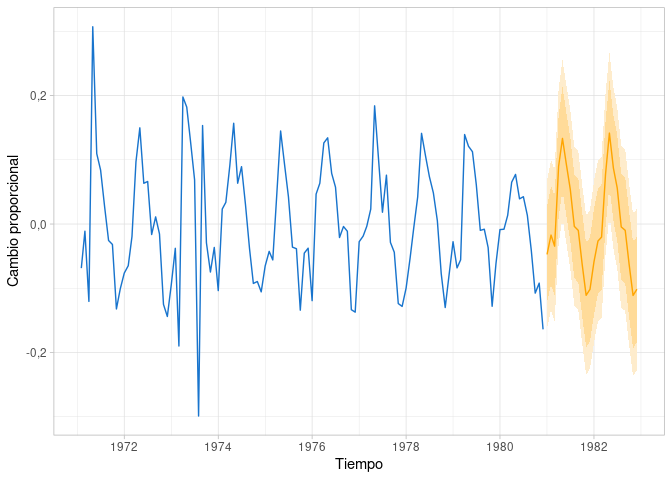
\includegraphics{/home/marcelo/MEGAsync/Msc-Math-Applied/Series Temporales/output/Lab-Session-8-FPP_files/figure-latex/forecast-plot-1} \end{center}

\hypertarget{predicciuxf3n-usando-suavizado-exponencial.}{%
\subsubsection{Predicción usando suavizado exponencial.}\label{predicciuxf3n-usando-suavizado-exponencial.}}

Ahora se ajusta un modelo usando suavizado exponencial, minimizando la sumatoria de cuadrados, usando solo componentes aditivos para la estacionalidad y la tendencia, obteniéndose un modelo con un RMSE de \text{0,054986} y MAE de \text{0,0371671}, comparables a los obtenidos para el modelo ajustado inicialmente, sin regresores, mostrado en la ecuación \eqref{eq:model}.
Los valores de AIC y BIC son un orden de magnitud mayor para el modelo ajustado usando ETS.

Los valores estimados para los parámetros de suavizados son: \(\alpha= \text{0,0062}\), \(\beta= \text{0,0001}\), y \(\gamma= \text{0,0087}\). Los valores tan pequeños para estos parámetros indican que el nivel, tendencia, y estacionalidad apenas varían con el tiempo.

Las predicciones se muestran en la figura \ref{fig:ets-forecast-plot}, junto con la predicción obtenida antes en la figura \ref{fig:forecast-plot} (linea gris a trozos), donde se observa que el modelo ETS ajustado predice de forma similar la serie durante los 24 meses siguientes.

\begin{Shaded}
\begin{Highlighting}[]
\KeywordTok{autoplot}\NormalTok{(cm_transf, }\DataTypeTok{colour=}\StringTok{"dodgerblue3"}\NormalTok{) }\OperatorTok{+}
\StringTok{    }\KeywordTok{autolayer}\NormalTok{(ets_forecast, }\DataTypeTok{colour=}\StringTok{"orange"}\NormalTok{) }\OperatorTok{+}
\StringTok{    }\KeywordTok{autolayer}\NormalTok{(forecast_}\DecValTok{24}\NormalTok{_month, }\DataTypeTok{level=}\OtherTok{NULL}\NormalTok{, }\DataTypeTok{colour=}\StringTok{"200"}\NormalTok{, }\DataTypeTok{linetype=}\DecValTok{2}\NormalTok{) }\OperatorTok{+}
\StringTok{    }\KeywordTok{scale_x_yearmonth}\NormalTok{(}\DataTypeTok{date_labels =} \StringTok{"%Y"}\NormalTok{) }\OperatorTok{+}
\StringTok{    }\KeywordTok{theme_light}\NormalTok{() }\OperatorTok{+}\StringTok{ }
\StringTok{    }\KeywordTok{xlab}\NormalTok{(}\StringTok{'Tiempo'}\NormalTok{) }\OperatorTok{+}\StringTok{ }\KeywordTok{ylab}\NormalTok{(}\StringTok{'Cambio proporcional'}\NormalTok{) }\OperatorTok{+}
\StringTok{    }\KeywordTok{theme}\NormalTok{(}\DataTypeTok{legend.position=}\StringTok{"none"}\NormalTok{)}
\end{Highlighting}
\end{Shaded}

\begin{center}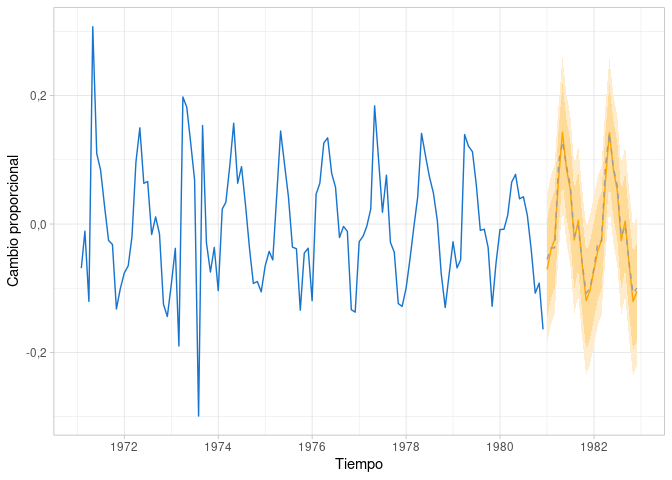
\includegraphics{/home/marcelo/MEGAsync/Msc-Math-Applied/Series Temporales/output/Lab-Session-8-FPP_files/figure-latex/ets-forecast-plot-1} \end{center}

\end{document}
